\chapter{An optimal approach for time series segmentation: Application to the supervised classification}
\label{seg}
%\minitoc
\section{Introduction}
Time series databases are often huge. This is particularly the case of the Large Synoptic Survey Telescope (LSST) database which records data from of telescopes \cite {lsst}. It has billions of time series (10 Petabytes). Another example is the  SACR-FRM project that uses sensors to measure the efforts of a  manual wheelchair user at a sample  frequency of 100 Hz \cite{SACR-FRM}. For instance :  ten minutes recording produce time series of 60 000 measurements. Faced to this, several scientific works were carried out with the aim of reducing the storage space of time series and accelerating their treatment.  A widely used approach is to change the representation of time series to reduce their length. This technique was introduced by Agrawal et al. \cite{Agrawal1993}; he uses the discrete Fourier transform to obtain a compact representation of the time series.
 Other methods have also been used: the decomposition in eigenvalue \cite{Wu1996}, the  discrete wavelet transform \cite{Chan1999} and the Piecewise Aggregate Approximate (PAA) \cite{keogh2001locally}. This last method has shown its effectiveness compared to the previous three ones because it is easier to understand, to implement, but also faster to execute and it allows to build indexes in linear time. PAA suggests to split the time series into segments of the same length, then to replace each segment by the average of its points. This method generates a compact representation, of time series composed with as few segments as possible that reduces space storage and processing time of time series.
 However, a too compact representation distorts the time series and causes a loss of information. How then to choose the right number of segments to consider? Our work is based on a simple observation: the use of the arithmetic average is relevant when the variance of the population is small as illustrated in figure \ref{fig:average22}.
 
 

\begin{figure}
\centering
\subfloat[]{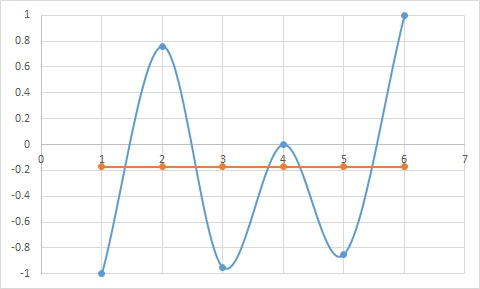
\includegraphics[scale=0.6]{moyenne_des_segment1.jpg}} \subfloat[]{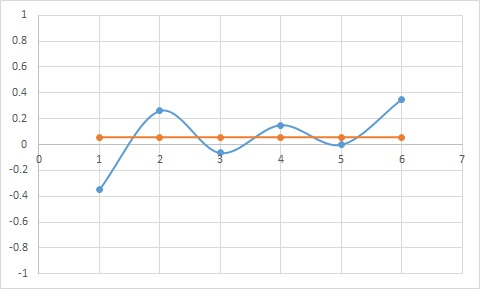
\includegraphics[scale=0.6]{moyenne_des_segment2.jpg}}
\caption{These figures show the average of two segments. In the first
case (a) the data points of the segment are far from the average, in the second case (b) they are close to the average. Replacing data points of a segment by their average introduces an error that the can be measured from the gap between the points and the average. }

\label{fig:average22}
\end{figure}


 
 
 We define here a minimal bound for the number of segments to be considered, and we propose an algorithm which allows choosing the number of segments which minimizes their mean squared error, with the aim to reduce the length of the time series without altering the information they contain.
 
 
  The rest of this appendix is organized as follows: the  section \ref{probleme22} presents a formal definition of our problem and an algorithm  to solve it; the section \ref{results} presents and comments the results of the experiments and the section \ref{conclusion} concludes the appendix and presents some perspectives for this work.
 

\section{Granularity of time series segments}
\label{probleme22}


\subsection{Notations and definitions}
\paragraph{Definition 1:} A \textbf{time series} or \textbf{time series}
$ X = x_{0}, x_{1}, \cdots, x_{m} $ is a sequence of numerical values representing the evolution of a specific quantity over time. $ x_{m} $ is the most recent value.

\begin{definition}
A segment $ X_{i} $ of length $ l $ of the time series
$ X $ of size $ m $ $ (l <m) $ is a sequence consisting of $ l $ consecutive variables
$ X $ beginning at the  position  $ i $  and ending at the position $ i + l-1 $.
We have: $ X_{i} = x_{i}, x_{i + 1}, ..., x_{i + l-1} $
\end{definition}

 
\begin{definition}
The arithmetic mean of the data points of a segment $ X_{i} $ of size $ l $ is
denoted $ \bar {X}_{i} $ and is defined by
	\begin{eqnarray}
		\bar{X}_{i} = \frac{1}{l} \sum_{j = 0}^{l-1} x_{i + j}.
	\end{eqnarray}

\end{definition}





\subsection{Information theory and minimum number of segments}
To mitigate the effects of noise during time series processing, Keogh and Kasetty \cite{KeoghBenchmarks} recommend that they are normalized. Normalizing the time series makes them compatible with a normal distribution \cite{Lin2007}. According to this method, 95 \% of the points in the time series are between plus and  minus two times the standard deviation $ (\sigma) $ and twice the standard deviation of the points, and thus 5 \% of the points of the series are outside this range. These points correspond to the ends of the series as shown in the figure \ref{standard_deviation}.


\begin{figure}
\centering
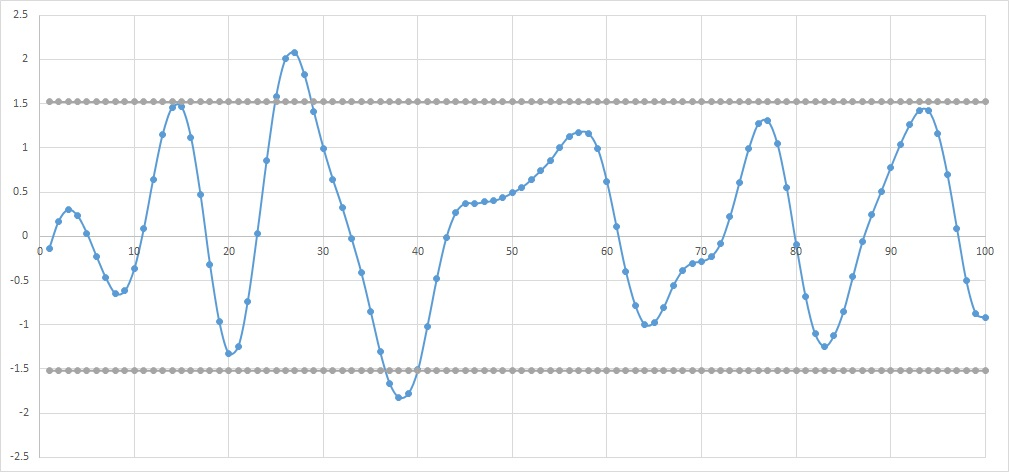
\includegraphics[scale = 0.50]{fordA_ecart-type}
\caption{This figure shows the first 100 points of the first time series  of the fordA dataset available in the UCR \cite{UCRArchive} database. Time series are normalized. The two horizontal lines delimit the interval corresponding to twice the standard deviation and minus two times the standard deviation of the points of the time series. We can observe that the points outside this range are at the ends of the time series.}
\label{standard_deviation} 
\end{figure}



\subsection{Notations and definitions}



\begin{definition}
The arithmetic mean of the data points of a segment $ X_{i} $ of size $ l $ is
denoted $ \bar {X}_{i} $ and is defined by :

\begin{eqnarray}
\bar{X}_{i} = \frac{1}{l} \sum_{j = 0}^{l-1} x_{i + j}.
\end{eqnarray}

\end{definition}




Also, information theory tells  that the amount of information relating to an event is equal to $ -log_{2}(p) $ where $ p $ is the probability of the event
\cite{Shannon2001} . In other words, a very likely event ($ p \longrightarrow1 $) brings less information than an unlikely event ($ p \longrightarrow0 $). Therefore, a point outside the interval $ [- 2 \sigma, + 2 \sigma] $ provides more information than a point within that range. Indeed, the probability that one point is in the range is $ 0.95$ while the probability that one point is out of range is $ 0.05 = \frac{1}{20} $ .


If we choose a minimum number $ (\alpha) $ of segments less than 5 \% of the length of the time series, we risk to aggregate the data points within the interval $ [- 2 \sigma, 2 \sigma] $ and those outside this range. This will have two consequences: firstly, this aggregation will alter the information carried by data points. Secondly, this aggregation will increase the variance of the segments obtained. So we chose to  consider 5\% of the number of points in the time series as the minimum number of segments. This allows us to define the following functions of $ \mathbb{N} \rightarrow \mathbb{N} $:

\begin{eqnarray}
\alpha: n \mapsto \alpha(n) = \left \{
\begin{array}{c}
\left \lfloor \frac{n}{20} \right \rfloor \: if \: \left \lfloor \frac{n}{20} \right \rfloor \geq 2 \\
2 \: otherwise
\end{array} 
\right.
\end{eqnarray}



\begin{eqnarray}
\beta: n \mapsto \beta(n) = \left \lfloor \frac{n}{2} \right \rfloor
\end{eqnarray}

 $ \beta $ gives the maximum number of segments. Indeed, a segment is made up of at least 2 points, so there is at most $ \left \lfloor
\frac{n}{2} \right \rfloor $ segments. The number of segments W that we will consider is greater than or equal to $ \alpha (| X |) $ and less than or equal to $ \beta (| X |) $. The next subsection explains how we choose the value of W.

\subsection{Minimize the squared error to choose the number of segments}
After dividing a time series into segments, we replace each segment by the average of the data points that constitute it. The variance between the points of each segment can be measured from the mean squared error. Our problem is therefore the following:
\paragraph{} Let $ X = x_{0}, x_{1}, \cdots, x_{n} $ a time series of size $ n $, look for $ W \in \mathbb{N} $ such that $ \alpha(n) \leq W \leq \beta(n) $ and 
\begin{eqnarray}
 \frac{1}{n} \sum_{i = 1}^{^{W}} \sum_{j = (i-1) k}^{ik} (\bar{X}_{i} - X_{j})^{2} 
\end{eqnarray}
 is minimal, where $ \bar{X}_{i} $ is the arithmetic mean of a segment of length $ k $. 




\paragraph{} To solve this problem, we
propose an algorithm that proceeds as follows:
\begin{enumerate}
\item For each value of W, with $ \alpha(n) \leq W \leq \beta(n) $
\begin{enumerate}
\item Calculate the squared error of each segment
$ X_{i} = x_{i}, x_{i + 1}, ..., x_{i + l-1}; $
\item Calculate the mean of the quadratic errors;
\end{enumerate}
\item The value of W returned is the one that produces a minimum average squared error. 
\end{enumerate}

These conditions are implemented in algorithm \ref{algo1}:

\begin{algorithm}[h]
\DontPrintSemicolon
\KwIn{length\_min, length\_max : repectively the minimal and the maximal length of a segment.\\ v : a time series}
\KwOut{The optimal number of segment to be use with Piecewise Aggregate approXimation}
\SetKwBlock{Begin}{function}{end function}

\Begin($\text{optimalNumberOfSegment} {(} length\_min, \, length\_max, \, v{)}$)
{
  $len\_v \leftarrow length(v)$\;
  $n \leftarrow length\_max - length\_min + 1$\;
  \ForAll{$i \in \{length\_min,...,length\_max\}$}
  {
    $x[j, 1] \leftarrow i$\;
    $z[j, 1] \leftarrow  (1/len\_v) * sum\_SSE(v, i)$\; \\computation of the error    
		$j \leftarrow j + 1$\;
  }
	$ind\_min \leftarrow indice\_minimun(z)$\;
  \Return{$floor(len\_v/x[ind\_min, 1])$}

}
\caption{optimalNumberOfSegment}
\label{algo1}
\end{algorithm}


%\begin{algorithm}
%\caption{longueur\_optimale (long\_min, long\_max, v)}
%\begin{algorithmic} 
%\STATE $len\_v \leftarrow length(v)$
%\STATE $n \leftarrow long\_max - long\_min + 1$
%\FOR{$(i\, in \,long\_min:long\_max)$} 
% \STATE $x[j, 1] \leftarrow i$
% \STATE $z[j, 1] \leftarrow  (1/len\_v) * somme\_SSE(v, i)$ //Calcul de l'erreur
% \STATE $j \leftarrow j + 1$
%%\ENDFOR
% \STATE $ind\_min \leftarrow indice\_minimun(z)$
%\RETURN $floor(len\_v/x[ind\_min, 1])$
%\end{algorithmic}
%\end{algorithm}


%\begin{algorithm}
%\caption{sum\_SSE (v, nbPoints)}
%\begin{algorithmic} 
%\STATE $n \leftarrow length(v)$
%\STATE $ind\_debut \leftarrow 1$
%\STATE $aux\_se \leftarrow c()$
%\STATE $tableau\_indice\_debut \leftarrow c()$
%\STATE $i \leftarrow 0$

%\WHILE{$(ind\_debut + nbPoints) \leq n$} 
%\STATE $tableau\_indice\_debut[i] \leftarrow ind\_debut$
%\STATE $ind\_debut \leftarrow ind\_debut + nbPoints$
%\STATE $i \leftarrow i + 1$
%\ENDWHILE

%\STATE $m \leftarrow length(tableau\_indice\_debut)$
%%\FOR{(i in 1:m) parallel loop} 
% \STATE $aux\_se[i] \leftarrow $
%\STATE$ SSE\_segment(v, nbPoints, tableau\_indice\_debut[i])$
%\ENDFOR
%\RETURN $somme(aux\_se)$
%\end{algorithmic}
%\end{algorithm}

\begin{algorithm}[h]
\DontPrintSemicolon
\KwIn{v : a time series.\\ nbPoints : the length of a segment}
\KwOut{The sum of squares error associated with a segment length}
\SetKwBlock{Begin}{function}{end function}

\Begin($\text{sum\_SSE} {(} v, \, nbPoints{)}$)
{
  $n \leftarrow length(v)$\;
	$ind\_debut \leftarrow 1$\;
	$aux\_se \leftarrow c()$\;
	$tab\_indices\_debut \leftarrow c()$\;
	$i \leftarrow 0$\;
	
	\While{$(ind\_debut + nbPoints) \leq n$}
	{
		$tab\_indices\_debut[i] \leftarrow ind\_debut$\;
		$ind\_debut \leftarrow ind\_debut + nbPoints$\;
		$i \leftarrow i + 1$\;
	}
	
	$m \leftarrow length(tab\_indices\_debut)$\;
	
	 \ForAll{$i \in \{1,...,m\}$}
  {
		$aux\_se[i] \leftarrow SSE\_segment(v, nbPoints, tab\_indices\_debut[i]) $\;
  }

  \Return{$sum(aux\_se)$}

}
\caption{sum\_SSE}
\label{algo2}
\end{algorithm}
 
 

\paragraph{Complexity of the algorithm}\\
The calculation of the squared error of a segment is done in $ O(\left \lfloor
\frac{n}{W} \right \rfloor) $.

The time complexity of calculating the mean squared error for segment splitting is
$ O(n). $


The number of segments varies from $ \left \lfloor \frac{n}{20} \right \rfloor, \; \left \lfloor \frac{n}{19} \right \rfloor $ \ldots $ \left \lfloor \frac{n}{2} \right \rfloor $. There are 19 possible divisions in segments. The time complexity of calculating the value of W which minimizes the error
mean squared is: $ 19 \times O(n) = O(n) $.


To exploit the compact representations of the time series, we must be able to compare them. The next subsection presents how to compare compact time series that we get.

\subsection{Dynamic Time Warping Algorithm and comparison of compact representations}

The Dynamic Time Warping algorithm (DTW)\cite{Keogh2004} allows to carry out a non-linear correspondence between two time series by minimizing the distance between them. It proceeds as follows:


Let $X$ and $Y$ be two time series;

\begin{eqnarray}
X=x_{1},x_{2},\cdots,x_{n};\\
Y=y_{1},y_{2},\cdots,y_{m}.
\end{eqnarray}


 To align them, the algorithm constructs a matrix $ n \times m $ where
the element $ (i, j) $ of the matrix corresponds to the square distance $ (x_{i} - y_{j}) ^ {2} $, which
is the alignment between $ x_{i} $ and $ y_{j} $. To find the best alignment between the two time series, we build
the path in the matrix that minimizes the sum of the square distances. This path is calculated by
dynamic programming from the following recurrence:

\begin{eqnarray}
\gamma(i, j) = d (x_{i}, y_{j}) + min \{\gamma(i-1, j-1), \gamma(i-1, j), \gamma(i , j-1) \},
\end{eqnarray}

where $ d(x_{i}, y_{j}) $ is the square of the distance contained in the cell $ (i, j) $ and $ \gamma(i, j) $ is the
cumulative distance at the position $ (i, j), $ which is calculated by the sum of the square of the distance to
the position $ (i, j) $ and the minimum cumulative distance of its three adjacent cells.


Piecewise Aggregate Approximation(PAA) provides Euclidean-based distance measurement to compare compact representations. However, we chose to use the Dynamic Time Warping algorithm for the following reasons:
\begin{enumerate}
\item PAA of the time series leads to temporal deformation. Indeed,
with two time series of length $ n $, we can apply our algorithm to the
 first time series, then reduce it to $ N_{1} $ segments and reduce the second to $ N_{2} $
 segments with $ N_{1} <N_{2} $.
\item The DTW algorithm  is known to have the best performance for sequence alignment in several :
in robotics, biometrics, music, climatology, aviation, gesture recognition, cryptanalysis, astronomy, exploration
space \cite{Rakthanmanon2012}.

\end{enumerate}


\section{Results and Discussion}
\label{results} 
 First, we present the datasets used during the experiment.
 Then we evaluate the performances of the proposed methods in terms of  length reduction  of time series and classification errors.

\subsection{Datasets}

We performed tests on 85 datasets that come from the UCR database
\cite{UCRArchive} . Detailed information on the datasets is presented in
the Table \ref{sets_of_data}.
 In the UCR database, each data set is divided into a learning set and a test set. Datasets contain between 2 and 60 classes and the time series of these datasets have lengths that range from 24 to 2709 points. The Table \ref{sets_of_data} presents a
 detailed description of the datasets. The following paragraph presents the assessment of the performance of our algorithm on these datasets.
 
\LTcapwidth=\textwidth
\begin{longtable}
   {|p{0.05\linewidth}|p{0.4\linewidth}|p{0.1\linewidth}|p{0.15\linewidth}|p{0.15\linewidth}|}
   \hline
	 \textbf{N} & \textbf{Name} &\textbf{Nb. of classes} &\textbf{Size of training set} &\textbf{Size of testing set}  \endfirsthead
   \hline
   \textbf{N} & \textbf{Name} &\textbf{Nb. of classes} &\textbf{Size of training set} &\textbf{Size of testing set}  \\
	 \hline
   \multicolumn{5}{|p{0.6666\linewidth}|}{Following ... } \\
   \hline
	 \endhead
   \hline
   \multicolumn{5}{|p{0.6666\linewidth}|}{Continue to the next page}\\ 
	 \hline 
	 \endfoot 
	 \hline
   \multicolumn{5}{|p{0.6666\linewidth}|}{End} \\
   \hline
   \endlastfoot 
	\hline
	
1 & 50Words  & 50  & 450  & 455 \\

2 & Adiac  & 37 & 390 & 391 \\

3 & ArrowHead  & 3 & 36 & 175\\

4 & Beef  & 5 & 30 & 30\\

5 & BeetleFly  & 2  & 20  & 20\\

6 & BirdChicken  & 2  & 20  & 20\\

7 & Car  & 4  & 60  & 60\\

8 & CBF & 3 & 30 & 900\\

9 & ChlorineConcentration  & 3  & 467  & 3840\\
 
10 & CinC\_ECG\_torso  & 4  & 40  & 1380\\

11 & Coffee  & 2  & 28  & 28 \\

12 & Computers  & 2  & 250  & 250\\

13 & Cricket\_X  & 12  & 390  & 390\\

14 & Cricket\_Y  & 12  & 390  & 390\\

15 & Cricket\_Z  & 12  & 390  & 390\\

16 & DiatomSizeReduction  & 4  & 16  & 306\\

17 & DistalPhalanxOutlineAgeGroup  & 3  & 139  & 400\\
 %& OutlineAgeGroup &  &  & \\

18 & DistalPhalanxOutlineCorrect & 2  & 276  & 600\\
 %& OutlineCorrect  &  &  & \\
 
19 & DistalPhalanxTW  & 6  & 139  & 400 \\

20 & Earthquakes  & 2  & 139 & 322 \\

21 & ECG & 2  & 100  & 100 \\

22 & ECG5000  & 5  & 500 & 4500\\

23 & ECGFiveDays & 2  & 23 & 861\\
24 & ElectricDevices  & 7  & 8926  & 7711\\

25 & Face (all)  & 14  & 560 1 & 690\\

26 & Face (four)  & 4  & 24  & 88\\
 
27 & FacesUCR  & 14  & 200  & 2050\\

28 & Fish & 7  & 175 & 175 \\

29 & FordA  & 2  & 1320 & 3601\\

30 & FordB  & 2  & 810  & 3636 \\

31 & Gun-Point  & 2  & 50  & 150 \\
 
32 & Ham  & 2  & 109 & 105\\
 
33 & HandOutlines  & 2  & 370 & 1000 \\
 
34 & Haptics  & 5  & 155  & 308 \\
 
35 & Herring  & 2 & 64 & 64 \\
 
36 & InlineSkate  & 7  & 100  & 550 \\

37 & InsectWingbeatSound  & 11  & 220  & 1980\\
 
38 & ItalyPowerDemand  & 2  & 67  & 1029 \\
 
39 & LargeKitchenAppliances  & 3  & 375  & 375 \\

40 & Lightning-2  & 2 & 60  & 61 \\
41 & Lightning-7  & 7  & 70  & 73 \\
 
42 & MALLAT & 8  & 55  & 2345\\
 
43 & Meat  & 3 & 60  & 60 \\
 
44 & MedicalImages  & 10  & 381  & 760\\

45 & MiddlePhalanxOutlineAgeGroup & 3  & 154  & 400 \\
 %& OutlineAgeGroup  &  &  & \\
 \ldots& \ldots  & \ldots & \ldots & \ldots \\
\caption{85 UCR  datasets used for experimental validation.
The full list is available in \cite{UCRArchive}}
\label{sets_of_data}
\end{longtable}



\subsection{Comparison of algorithm performance}
% Visionner le code LaTeX du paragraphe 21
Table \ref{erreur_classification} presents the comparison
of the classification error of 1-Nearest Neighbor (1-NN) algorithms associated with Euclidean  distance (col.4), 1-NN, associated with the DTW algorithm using a constraint (a deformation window) (col.5), 1-NN associated with the algorithm of unconstrained dynamic time warping (DTW) applied to the raw data (6) and the 1-NN algorithm associated with DTW applied to the data pre-processed by our algorithm  (7). The $ (col.4) $ algorithm gives the best results that are to say
$ ((col.4) \leq (col.5) \: and \:(col.4) \leq (col.6) \: and \:(col.4) \leq (col.7)) $ on $ 20 $ datasets, the algorithm $ (col.5) $ is the best on $ 47 $ datasets, the $ (col.6) $ algorithm is the best on $ 21 $ datasets, the $ (col.7) $ algorithm is the best on $ 21 $ datasets. Although none of these algorithms have the best performance on all datasets, the algorithm $ (col.5) $ averaged the smallest misclassification \textbf{0.237} and the most expensive $ (col.4) $ algorithm the largest average error \textbf{0,288}.
The $ (col.6) $ and $ (col.7) $ algorithms have relatively close average error rates  equal to \textbf{0,256} and \textbf{0,258} respectively.


To evaluate the effects of the \textbf{change of representation} of the time series on their
\textbf{classification}, we compared the length of the time series and the errors of
classification presented by the columns $ (6) $ and $ (7) $ of Table  \ref{erreur_classification}.
Indeed, these two columns use the same 1-NN classification algorithm and the same 
distance function DTW. The only difference between these columns is the nature of the data: the $ (6) $ column
uses the raw data and the column $ (7) $ the compacted data with the method described above. The result of the comparison between these two columns can be resumed as follows:

\begin{itemize}
\item Regarding the length of the time series; the $ (6) $ algorithm uses all the points of
the time series. On the other hand, the $ (7) $ algorithm uses compact representations whose
length varies between \textbf{15} \% and \textbf{34} \% of the initial length of the time series.
On average, the compact representations have a length equal to \textbf {20} \% of the initial time series
\item For classification errors, the error $ (7)> (6) $ on 40 datasets,
the error of $ (7) = (6) $ on 3 datasets and the error of $ (7) <(6) $ on 42 datasets.
\end {itemize}

 These results are encouraging because, despite the reduction in the length of the time series
 errors, the classification error with the compact representation is less than or equal to
that of the raw data classification for 45 datasets out of the 85 available in the
UCR base. These results are summarized in Figure \ref{synthesis}. One of the reasons for this observed improvement over 42 datasets is as follows: the DTW algorithm  is sensitive to noise, therefore by aggregating the points of the segments, we reduce the effects of noise.


% Visionner le code LaTeX du paragraphe 29

\begin{figure}
\center
\subfloat[]{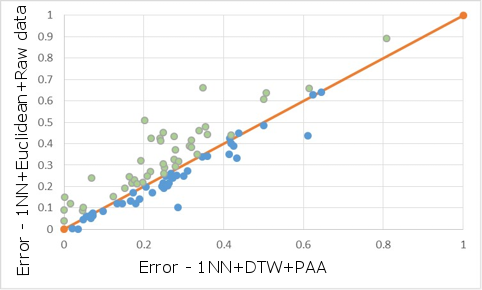
\includegraphics[scale=0.50]{erreur_dtw-reduit_euclid2.png} }
\subfloat[]{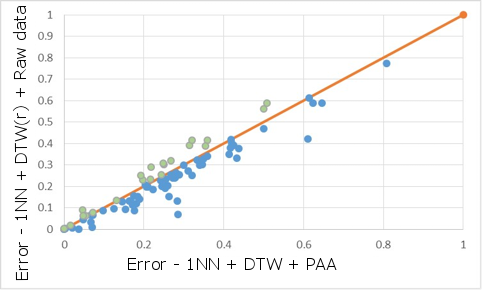
\includegraphics[scale=0.50]{erreur_dtw-reduit_dtw(r)2.png}}\\
\subfloat[]{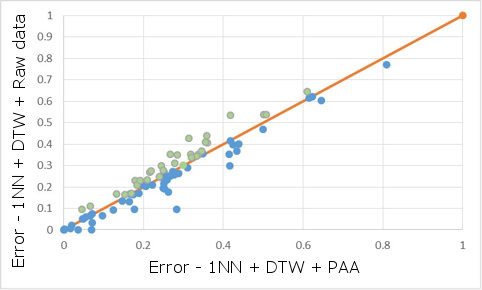
\includegraphics[scale=0.50]{erreur_dtw-reduit_dtw2.png}}

\caption{Two-by-two comparison of the classification errors of the algorithm
1-Nearest Neighbor (1-NN) using Euclidean distance with 1-NN using two variations of the temporal warping algorithm on raw data
 and compact data}

\label{synthesis}

\end{figure}



\begin{longtable}
   {|p{0.05\linewidth}|p{0.1\linewidth}|p{0.1\linewidth}|p{0.1\linewidth}|p{0.15\linewidth}|p{0.1\linewidth}|p{0.1\linewidth}|}
   \hline
	 \textbf{(1)} &\textbf{(2)} &\textbf{(3)} &\textbf{(4)} &\textbf{(5)} &\textbf{(6)} &\textbf{(7)} \endfirsthead
   \hline
   \textbf{(1)} &\textbf{(2)} &\textbf{(3)} &\textbf{(4)} &\textbf{(5)} &\textbf{(6)} &\textbf{(7)} \\
	 \hline
   \multicolumn{7}{|p{0.6666\linewidth}|}{Following ... } \\
   \hline
	 \endhead
   \hline
   \multicolumn{7}{|p{0.6666\linewidth}|}{Continue to the next page}\\ 
	 \hline 
	 \endfoot 
	 \hline
   \multicolumn{7}{|p{0.6666\linewidth}|}{End} \\
   \hline
   \endlastfoot 
	\hline
	
1  & 54  & 0,20  & 0,369   & 0,242 (6)  & 0,31  & \textbf{\emph{0,279}}\\
2  & 35  & 0,20  & \emph{0,389 } & 0,391 (3)  & \textbf{0,396 } & 0,425\\
3  & 50  & 0,20  & \emph{0,2 } & \emph{0,200 (0) } & 0,297  & \textbf{0,246}\\
4  & 78  & 0,17  & \emph{0,333} & \emph{0,333 (0) } & \textbf{0,367 } & 0,433\\
5  & 85  & 0,17  & \emph{0,25 } & 0,300 (7)  & 0,3  & \textbf{0,300}\\
6  & 85  & 0,17  & 0,45  & 0,300(6)  & \emph{0,25 } & \textbf{\emph{0,250}}\\
7  & 96  & 0,17 & 0,267  & 0,233 (1)  & 0,267  & \textbf{\emph{0,217}}\\
8  & 32  & 0,25  & 0,148   & 0,004 (11)  & 0,003  & \textbf{\emph{0,002}}\\
9  & 33  & 0,20 & \emph{0,35 } & \emph{0,35 (0) } & \textbf{0,352 } & 0,414\\
10  & 234  & 0,14  & 0,103  & \emph{0,07 (1)}  & 0,349  & \textbf{0,285}\\
11  & 57  & 0,20  & \emph{0 } & \emph{0,000 (0)} & \textbf{\emph{0 }} & 0,036\\
12  & 120  & 0,17  & 0,424  & 0,380 (13)  & \textbf{\emph{0,3 }} & 0,416\\
13  & 60  & 0,20  & 0,423  & 0,228 (10)  & 0,246  & \textbf{\emph{0,241}}\\
14  & 60  & 0,20  & 0,433  & \emph{0,238 (17) } & \textbf{0,256}  & 0,277\\
15 & 60  & 0,20  & 0,413  & 0,254 (5)  & 0,246  & \textbf{\emph{0,244}}\\
16  & 69  & 0,20  & 0,065  & 0,065 (0)  & \textbf{\emph{0,033}} & 0,072\\
17  & 20  & 0,25  & 0,218  & 0,228 (1)  & 0,208  & \textbf{\emph{0,198}}\\
18  & 20  & 0,25  & 0,248  & \emph{0,232 (2) } & \textbf{\emph{0,232}}\emph{ } & 0,255\\
19  & 20  & 0,25  & 0,273  & \emph{0,272 (0) } & \textbf{0,29 } & 0,310\\
20  & 85  & 0,17  & 0,326  & \emph{0,258 (22) } & \textbf{\emph{0,258 }} & 0,276\\
21  & 24  & 0,25  & \emph{0,12 } & \emph{0,120 (0)} & 0,23  & \textbf{0,180}\\
22  & 35  & 0,25  & 0,075  & 0,075 (1)  & 0,076  & \textbf{\emph{0,072}}\\
23  & 34  & 0,25  & \emph{0,203 } & \emph{0,203 (0) } & \textbf{0,232 } & 0,259\\
24  & 24  & 0,25  & 0,45  & \emph{0,376 (14)}  & \textbf{0,399 } & 0,438\\
25  & 32  & 0,24  & 0,286   & \emph{0,192 (3) } & \textbf{\emph{0,192}} & 0,253\\
26  & 70  & 0,20  & 0,216   & \emph{0,114 (2)}  & 0,17  & \textbf{0,170}\\
27  & 32  & 0,24  & 0,231  & \emph{0,088 (12)}  & \textbf{0,095 } & 0,177\\
28  & 77  & 0,17  & 0,217  & \emph{0,154(4) } & \textbf{0,177}  & 0,263\\
29  & 83  & 0,17  & \emph{0,341 } & \emph{0,341 (0)} & 0,438  & \textbf{0,359}\\
30  & 83  & 0,17  & 0,442  & 0,414 (1) & 0,406  & \textbf{\emph{0,360}}\\
31  & 30  & 0,20  & 0,087   & 0,087 (0)  & 0,093 & \textbf{\emph{0,047}}\\
32  & 71  & 0,16  & \emph{0,4 } & \emph{0,400 (0) } & 0,533 & \textbf{0,419}\\
33  & 387  & 0,14 & 0,199  & \emph{0,197 (1) } & \textbf{0,202 } & 0,206\\
34  & 182  & 0,17  & 0,63 & \emph{0,588 (2)}  & 0,623  & \textbf{0,623}\\
35  & 85  & 0,17  & 0,484  & \emph{0,469 (5) } & \textbf{\emph{0,469 }} & 0,500\\
36  & 268  & 0,14 & 0,658 & \emph{0,613 (14)}  &  0,616 & \textbf{0,615}\\
37  & 51  & 0,20  & 0,438  & \emph{0,422 (2) } & 0,645 & \textbf{0,611}\\
38  & 8  & 0,33 & \emph{0,045} & \emph{0,045 (0)} & 0,05  & \textbf{0,048}\\
39  & 120  & 0,17 & 0,507 & 0,205 (94) & 0,205 & \textbf{\emph{0,203}}\\
40 & 106 & 0,17  & 0,246 & \emph{ 0,131 (6)} & \textbf{\emph{0,131}} & 0,164 \\
41 & 63  & 0,20 & 0,425  &  0,288 (5) & 0,274  & \textbf{\emph{0,219}}\\
42  & 170 & 0,17 & 0,086 & 0,086 (0) & \textbf{\emph{0,066}} & 0,097\\
43  & 74 & 0,17 & \emph{0,067 } & \emph{0,067 } & \emph{(0) 0,067} & \textbf{\emph{0,067}}\\
44  & 24 & 0,24  & 0,316  & \emph{0,253 (20)} & \textbf{0,263 } & 0,288\\
45  & 20  & 0,25  & 0,26  & 0,253 (5)  & \textbf{\emph{0,25}} & 0,268\\
46 & 20  & 0,25 & \emph{0,247}  & 0,318 (1) & 0,352  & \textbf{0,268}\\
47  & 20 & 0,25 & 0,439  & 0,419 (2)  & \textbf{\emph{0,416 }} & 0,419\\
48  & 21  & 0,25 & \emph{0,121} & 0,134 (1)  & 0,165  & \textbf{0,133}\\
49  & 125  & 0,17  & \emph{0,171} & 0,185 (1)  & \textbf{0,209} & 0,222 \\
50  & 125 & 0,17  & \emph{0,12 } & 0,129 (1) & \textbf{0,135} & 0,146\\
51  & 95  & 0,17 & \emph{0,133 } & \emph{0,133 (0) } & 0,167  & \textbf{0,167}\\
52  & 71  & 0,17 & 0,479   & 0,388 (7)  & 0,409  & \textbf{\emph{0,355}}\\
53  & 20  & 0,25 & \emph{0,239 } & \emph{0,239 (0) } & \textbf{0,272}  & 0,273\\
54  & 170  & 0,17  & 0,891  & 0,773 (14)  & \textbf{\emph{0,772 }} & 0,809\\
55  & 36  & 0,25  & 0,038 & \emph{0,000 (6)} & \emph{0 } & \textbf{\emph{0,000}}\\
56  & 20  & 0,25  & 0,215 & 0,215 (0)  & \textbf{\emph{0,195 }} & 0,249\\
57  & 20 & 0,25  & \emph{0,192} & 0,210 (1) & \textbf{0,216 } & 0,251\\
58  & 20  & 0,25  & 0,292 & \emph{0,263 (6) } & \textbf{\emph{0,263}} & 0,280\\
59  & 120  & 0,17  & 0,605 & 0,560 (8)  & 0,536 & \textbf{\emph{0,501}}\\
60  & 120  & 0,17  & 0,64  & \emph{0,589 (17) } & \textbf{0,603 } & 0,645\\
61  & 83 & 0,17  & 0,461 & \emph{0,300 (3) } & 0,35  & \textbf{0,339}\\
62  & 85  & 0,17  & 0,248  & 0,198 (4) & 0,232  & \textbf{\emph{0,210}}\\
63  & 120  & 0,17  & 0,659  & \emph{0,328 (15)}  & 0,357  & \textbf{0,349}\\
64  & 17  & 0,24  & 0,305  & 0,305 (0)  & 0,275 & \textbf{\emph{0,250}}\\
65  & 16 & 0,25  & \emph{0,141 } & \emph{0,141 (0) } & \textbf{0,169 } & 0,189 \\
66 & 170  & 0,17  & 0,151  & 0,095 (16)  & \textbf{\emph{0,093}} & 0,124\\
67  & 47  & 0,20  & 0,062  & 0,062 (0) & 0,06  & \textbf{\emph{0,055}}\\
68  & 32  & 0,25 & 0,211   & \emph{0,154 (2)} & 0,208 & \textbf{0,184}\\
69  & 79  & 0,20  & 0,1 & 0,062 (8) & 0,05  & \textbf{\emph{0,048}}\\
70  & 15  & 0,25  & 0,12   & 0,017 (6)  & \textbf{\emph{0,007}} & 0,017\\
71  & 55  & 0,20  & 0,32 & 0,250 (8)  & 0,228  & \textbf{\emph{0,193}}\\
72  & 68  & 0,20  & 0,192  & \emph{0,092 (5) } & 0,162 & \textbf{0,154}\\
73  & 55 & 0,20 & 0,24 &  0,010 (3) & \textbf{\emph{0 }} & 0,070 \\
74  & 32  & 0,25  & 0,09  &  0,002 (4) & \emph{0 } & \textbf{\emph{0,000}}\\
75  & 20 & 0,24  & 0,253  & 0,132 (5)  & \textbf{\emph{0,096 }} & 0,283\\
76  & 63 & 0,20 & 0,261  & 0,227 (4)  & 0,273  & \textbf{\emph{0,252}}\\
77  & 63 & 0,20  & 0,338  & \emph{0,301 (4)}  & 0,366 & \textbf{0,346}\\
78  & 63  & 0,20 & 0,35 & \emph{0,322 (6) } & 0,342  & \textbf{0,334}\\
79  & 157  & 0,17 & 0,052 & \emph{0,034 (4) } & 0,108  & \textbf{0,067}\\
80  & 30 & 0,20  & 0,005  &  0,005 (1) & \textbf{\emph{0,02}} & 0,021\\
81  & 46  & 0,20  & 0,389 & 0,389 (0)  & 0,426  & \textbf{\emph{0,315}}\\
82  & 54  & 0,20  & 0,382 & \emph{0,252 (8) } & 0,351 & \textbf{0,320}\\
83 & 150  & 0,17 & 0,635 & 0,586 (3)  & 0,536 & \textbf{\emph{0,508}}\\
84  & 150  & 0,17  & 0,414  & 0,414 (9)  & 0,337  & \textbf{\emph{0,320}}\\
85  & 71  & 0,17  & 0,17  & \emph{0,155 (2)} & \textbf{0,164 } & 0,174\\
\hline
$\bar{X}$  &   &   & 0,288 & 0,237 & 0,256 & 0,258\\
$\sigma$  &   &   & 0,175 & 0,161 & 0,166 & 0,160\\

\caption{ Column \textbf{(1)}  presents \textbf{numbers} of the datasets. Column  \textbf{(2)} the \textbf{reduced length} of the time series. Column \textbf{(3)} is the \textbf{ratio} of the length of the reduced time series over the length of the initial time series. Column \textbf{(4)}  designates the \textbf{1-Nearest Neighbor} algorithm, associated to the \textbf{Euclidean distance}. Column \textbf{(5)}  designates the algorithm of \textbf{1- Nearer Neighbor}, associated with the algorithm of \textbf{dynamic dynamic temporal deformation} using a \textbf{constraint} called deformation window that allows to stop the comparison of time series when one perceives that they are very different. Column \textbf{(6)}  represents  \textbf{1-Nearest Neighbor} algorithm  associated to the \textbf{unconstrained dynamic time warping} applied to the \textbf{raw data}.   Column \textbf{(7)} represents the \textbf{algorithm. 1-Nearest Neighbor} associated with the \textbf{dynamic time warping algorithm without constraints}, applied on the \textbf{compact representations} produced by our algorithm. We firstly compare, the classification error of the algorithms of columns(6) and (7) the smallest error is in \textbf{bold}. Then we compare the classification errors of algorithms of columns(4), (5), (6) and (7) the smallest error is put \textbf{italics}.}

\label{erreur_classification}
\end{longtable}


\section{Conclusion}

The purpose of this appendix was to propose an algorithm for choosing the number of segments to consider for the compact representation of a time series. In that aim, we have defined a minimum bound for the number of segments to be considered which is equal to 5 \% of the length of the time series. We have proposed an algorithm that chooses the number W of segments minimizing the mean squared error. Results of experiments conducted on 42 datasets
 have shown that the number of segments chosen allows two improvements:
 \begin{itemize}
\item IT significantly reduces the length of the time series; time series of reduced size have a length
which varies between $ 15 \% $ and $ 34 \% $ of the initial time series length
\item It improves supervised classification results on a set of 85 datasets
used in the literature. 
\end{itemize}
As a perspective for this work, we plan to vary the number of
segments W from $ 2 $ to $ \frac{n}{2} $ to see if our value of W is optimum for a task classification. We also plan to compare the results of this compact representation to
those of other representations used in the literature. We also plan to parallelize our algorithm to calculate the right number of segments in linear time. This work allows
reducing the storage space and the processing time of the time series. It also allows choosing the number of segments to consider when designing symbolic representation 
 of time series. Indeed, several symbolic representations of series
of the literature (SAX \cite{lin2003symbolic}, ESAX \cite{lkhagva2006extended}, 1d-SAX \cite{Malinowski2013},
SAX-TD \cite{sun2014improvement}, SAX-P \cite{siyou2015}) use the division into segments recommended by PAA.
\label{conclusion}



















\chapter{Determination of the probability density function of  uncertainty}
\label{pdf_uncertainty}
\minitoc

\section{Empirical probability distribution of residuals}
\paragraph{ descriptive statistics}

\begin{table}[h]
\centering
\caption{descriptive statistic}
\label{my-label}
\begin{tabular}{|c|c|c|c|c|c|}
\hline
\textbf{Min.} & \textbf{1st Qu.} & \textbf{Median} & \textbf{Mean} & \textbf{3rd Qu.} & \textbf{Max.} \\ \hline
-24.15        & -0.4735          & 0               & 0.2416        & 0.78             & 25.4          \\ \hline
\end{tabular}
\end{table}

\begin{figure}[h]
\centering
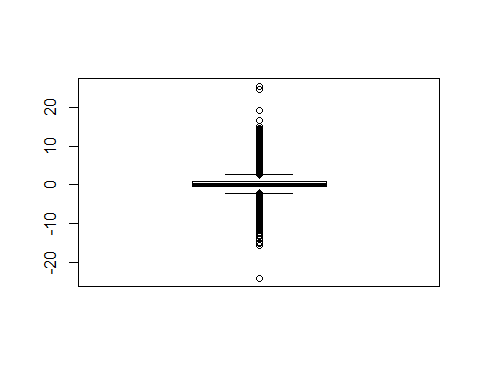
\includegraphics[scale=0.6]{box_plot}
\caption{Distribution of data around the mean}
\label{fig:average}
\end{figure}
35.65\% of values of uncertainty are equal  to zero


\paragraph{Distribution}
\begin{figure}[h]
\centering
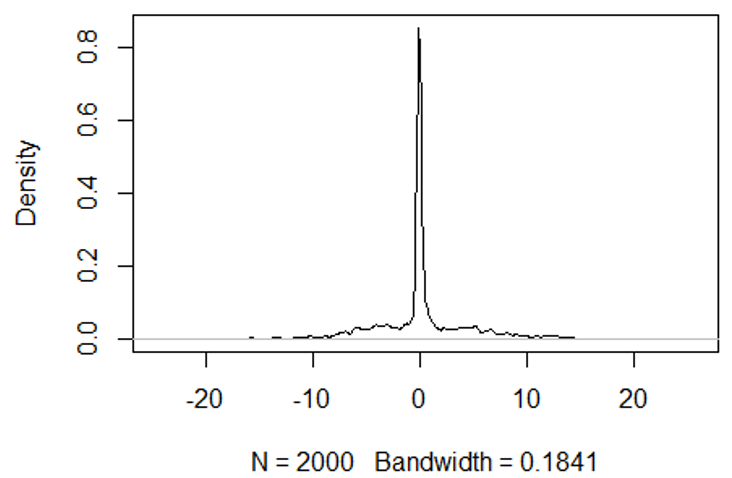
\includegraphics[scale=0.5]{ampiric_pdf}
\caption{Estimated probability density of data}
\label{fig:average}
\end{figure}

A priori the empirical probability density function does not allow   to know which probability law follows the residuals (uncertainty). To determine this, we  used statistical tests. The principle of statistical tests is as follows: we assume that the residues follow a defined probability law, and we calculate a p-value. If it is less than 0.05, the above hypothesis is rejected. Another method  is to hypothesize that the data follow a particular law and to estimate the parameters that best fit the law. If the theoretical probability density function estimated is closed to the empirical one, we assume that  the probability law follows by residuals is found.


\section{Theorical probability distribution}

Residuals are real values between minus infinity and plus infinity. The probability laws that residuals can follow are therefore:

\begin{itemize}
\item A normal law;
\item A law of Cauchy;
\item A Student's law t;
\item A general exponential law;
\item A double exponential law;
\item Generalized error distribution (GED);
\item A Pearson law type 4;
\item A generalization of the Student's law.
\end{itemize}


\paragraph{Normality test}:
For each tests in (Table \ref{normal}), the p-value is significant, so the sample does not follow a normal distribution.

\begin{table}[h]
\centering
\caption{normality test show that residues (uncertainty) do not follow normal law.}
\label{normal}
\begin{tabular}{llll}
\textbf{Test}    & Kolmogorov-Smirnov & Anderson-Darling  & Shapiro-Wilk      \\
\textbf{p-value} & \textless 2.2e-16  & \textless 2.2e-16 & \textless 2.2e-16
\end{tabular}
\end{table}

\paragraph{Cauchy's Law Test}: The Q-Qplot line does not match correctly with the data particularly the two extremities of the diagram (Fig. \ref{cauchy}); we can say that the data probably do not follow a Cauchy's law.

\begin{figure}[h]
\centering
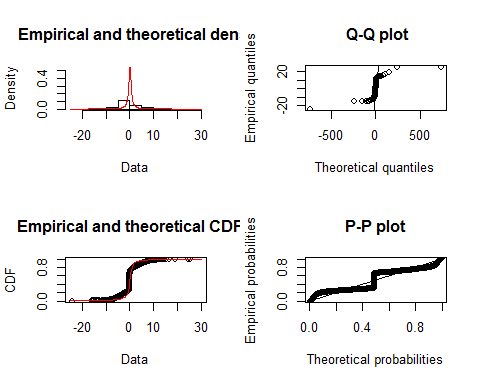
\includegraphics[scale=0.8]{cauchy}
\caption{Estimated probability density of data for Cauchy's law}
\label{cauchy}
\end{figure}

\paragraph{Student's Law test:} The Quantile-Quantile diagram, from the distribution function, does not match correctly the data, particularly the two extremities of the diagram (Fig. \ref{student}). We can then say that the data do not follow a Student's law.

\begin{figure}[h]
\centering
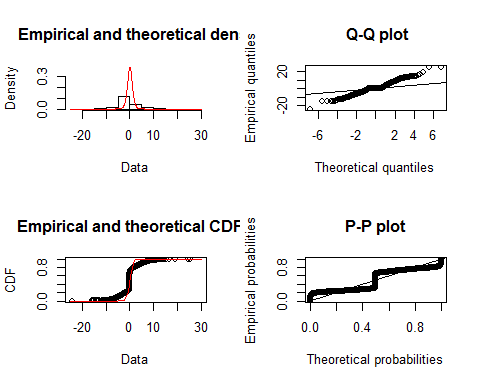
\includegraphics[scale=0.8]{student}
\caption{Estimated probability density of data for Student's law}
\label{student}
\end{figure}

\paragraph{Logistics law:} The probability density function matches the data reasonably well(Fig. \ref{logistic}), so we can say that the \textbf{residuals (uncertainty) follow a zero-inflated logistic law}.

\begin{figure}[h]
\centering
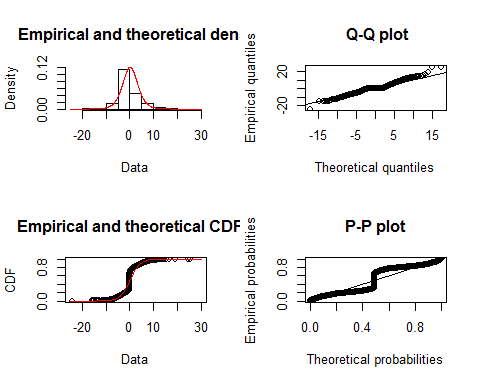
\includegraphics[scale=0.8]{logistic}
\caption{Estimated probability density of data for Logistic law}
\label{logistic}
\end{figure}









\chapter{Training and changes on propulsion technics}
\label{training_technic}
In this section, we want to evaluate the effect of the experiment on the propulsion technique used by manual wheelchair users. We assume that the shape of the $M_z$ moment of the left and right wheels reflects the propulsion technique used. Thus, in this paragraph, rather than using an approach that uses cycle properties, we  directly compared time series from a distance function while taking into account the presence of uncertainty in measurements. To do this, we applied FOTS-UShapelet to the measurements made and we deliver here the analysis we made of the results obtained.



FOTS-UShapelet was applied to the time series from the measurement of efforts made by eight valid subjects during the first week of use and after three weeks of use of the Manual Wheelchair. Table \ref{technic} details the obtained results. From the shape of the time series, we could form three large groups that correspond to three techniques that we have named T1, T2 and T3. For each subject of the experiment, we observe a difference between the propulsion techniques used at the beginning of the trial period and after three weeks. For example the subject SA01  uses the T1 technique 83\% and the T3 technique 17\% of the time during the first week. However, after three weeks of using the Manual Wheelchair, he uses the T1 technique 33\% of the time and the T3 technique 67\% of the time. So there is a change in the way he moves. 
However, the observed changes  vary according to the subjects (Table \ref{technic}). The variations in the evolution of propulsion techniques require personalized monitoring of locomotion and highlight the importance of using a Wheelchair Ergometer when learning locomotion in a Manual Wheelchair.




\begin{longtable}
   {|p{0.1\linewidth}|p{0.1\linewidth}|p{0.1\linewidth}|p{0.1\linewidth}|p{0.1\linewidth}|p{0.1\linewidth}|p{0.1\linewidth}|p{0.1\linewidth}|}
   
   \hline
\textbf{Subject} & \textbf{Week} & \textbf{Trial} & \textbf{wheel} & \textbf{technic} & \textbf{T1} & \textbf{T2} & \textbf{T3}\endfirsthead 
 \hline

\textbf{Subject} & \textbf{Week} & \textbf{Trial} & \textbf{wheel} & \textbf{technic} & \textbf{T1} & \textbf{T2} & \textbf{T3}  \\

	 \hline
   \multicolumn{8}{|p{0.8\linewidth}|}{Following ... } \\

   \hline
	 \endhead

   \hline
   \multicolumn{8}{|p{0.8\linewidth}|}{Continue to the next page}\\ 

	 \hline 
	 \endfoot 

	 \hline
   \multicolumn{8}{|p{0.8\linewidth}|}{End} \\

   \hline
   \endlastfoot 
	\hline
	
SA01NE           & T0S           & ES1            & RD             & 1                &             &             &             \\ \hline
SA01NE           & T0S           & ES1            & RG             & 1                &             &             &             \\ \hline
SA01NE           & T0S           & ES2            & RD             & 1                &             &             &             \\ \hline
SA01NE           & T0S           & ES2            & RG             & 3                &             &             &             \\ \hline
SA01NE           & T0S           & ES3            & RD             & 1                &             &             &             \\ \hline
SA01NE           & T0S           & ES3            & RG             & 1                & 0,83        & 0,00        & 0,17        \\ \hline
                 &               &                &                &                  &             &             &             \\ \hline
SA01NE           & T3S           & ES1            & RD             & 1                &             &             &             \\ \hline
SA01NE           & T3S           & ES1            & RG             & 3                &             &             &             \\ \hline
SA01NE           & T3S           & ES2            & RD             & 3                &             &             &             \\ \hline
SA01NE           & T3S           & ES2            & RG             & 1                &             &             &             \\ \hline
SA01NE           & T3S           & ES4            & RD             & 3                &             &             &             \\ \hline
SA01NE           & T3S           & ES4            & RG             & 3                & 0,33        & 0,00        & 0,67        \\ \hline
                 &               &                &                &                  &             &             &             \\ \hline
                 &               &                &                &                  &             &             &             \\ \hline
SA02GG           & T0S           & ES1            & RD             & 3                &             &             &             \\ \hline
SA02GG           & T0S           & ES1            & RG             & 1                &             &             &             \\ \hline
SA02GG           & T0S           & ES2            & RD             & 3                &             &             &             \\ \hline
SA02GG           & T0S           & ES2            & RG             & 3                & 0,25        & 0,00        & 0,75        \\ \hline
                 &               &                &                &                  &             &             &             \\ \hline
SA02GG           & T3S           & ES1            & RD             & 1                &             &             &             \\ \hline
SA02GG           & T3S           & ES1            & RG             & 1                &             &             &             \\ \hline
SA02GG           & T3S           & ES2            & RD             & 3                &             &             &             \\ \hline
SA02GG           & T3S           & ES2            & RG             & 1                &             &             &             \\ \hline
SA02GG           & T3S           & ES3            & RD             & 3                &             &             &             \\ \hline
SA02GG           & T3S           & ES3            & RG             & 3                & 0,50        & 0,00        & 0,50        \\ \hline
                 &               &                &                &                  &             &             &             \\ \hline
                 &               &                &                &                  &             &             &             \\ \hline
SA03JM           & T0S           & ES1            & RD             & 1                &             &             &             \\ \hline
SA03JM           & T0S           & ES1            & RG             & 1                &             &             &             \\ \hline
SA03JM           & T0S           & ES2            & RD             & 3                &             &             &             \\ \hline
SA03JM           & T0S           & ES2            & RG             & 1                &             &             &             \\ \hline
SA03JM           & T0S           & ES3            & RD             & 2                &             &             &             \\ \hline
SA03JM           & T0S           & ES3            & RG             & 1                & 0,67        & 0,17        & 0,17        \\ \hline
                 &               &                &                &                  &             &             &             \\ \hline
SA03JM           & T3S           & ES1            & RD             & 1                &             &             &             \\ \hline
SA03JM           & T3S           & ES1            & RG             & 3                &             &             &             \\ \hline
SA03JM           & T3S           & ES2            & RD             & 1                &             &             &             \\ \hline
SA03JM           & T3S           & ES2            & RG             & 1                &             &             &             \\ \hline
SA03JM           & T3S           & ES3            & RD             & 1                &             &             &             \\ \hline
SA03JM           & T3S           & ES3            & RG             & 1                & 0,83        & 0,00        & 0,17        \\ \hline
                 &               &                &                &                  &             &             &             \\ \hline
                 &               &                &                &                  &             &             &             \\ \hline
SA04BD           & T0S           & ES1            & RD             & 3                &             &             &             \\ \hline
SA04BD           & T0S           & ES1            & RG             & 1                &             &             &             \\ \hline
SA04BD           & T0S           & ES2            & RD             & 3                &             &             &             \\ \hline
SA04BD           & T0S           & ES2            & RG             & 1                &             &             &             \\ \hline
SA04BD           & T0S           & ES4            & RD             & 3                &             &             &             \\ \hline
SA04BD           & T0S           & ES4            & RG             & 3                & 0,33        & 0,00        & 0,67        \\ \hline
                 &               &                &                &                  &             &             &             \\ \hline
SA04BD           & T3S           & ES1            & RD             & 1                &             &             &             \\ \hline
SA04BD           & T3S           & ES1            & RG             & 3                &             &             &             \\ \hline
SA04BD           & T3S           & ES2            & RD             & 1                &             &             &             \\ \hline
SA04BD           & T3S           & ES2            & RG             & 1                &             &             &             \\ \hline
SA04BD           & T3S           & ES3            & RD             & 1                &             &             &             \\ \hline
SA04BD           & T3S           & ES3            & RG             & 1                & 0,83        & 0,00        & 0,17        \\ \hline
                 &               &                &                &                  &             &             &             \\ \hline
                 &               &                &                &                  &             &             &             \\ \hline
SA05AT           & T0S           & ES2            & RD             & 3                &             &             &             \\ \hline
SA05AT           & T0S           & ES2            & RG             & 1                &             &             &             \\ \hline
SA05AT           & T0S           & ES3            & RD             & 3                &             &             &             \\ \hline
SA05AT           & T0S           & ES3            & RG             & 3                &             &             &             \\ \hline
SA05AT           & T0S           & ES4            & RD             & 2                &             &             &             \\ \hline
SA05AT           & T0S           & ES4            & RG             & 1                & 0,33        & 0,17        & 0,50        \\ \hline
                 &               &                &                &                  &             &             &             \\ \hline
SA05AT           & T3S           & ES1            & RD             & 2                &             &             &             \\ \hline
SA05AT           & T3S           & ES1            & RG             & 2                &             &             &             \\ \hline
SA05AT           & T3S           & ES2            & RD             & 1                &             &             &             \\ \hline
SA05AT           & T3S           & ES2            & RG             & 3                &             &             &             \\ \hline
SA05AT           & T3S           & ES3            & RD             & 2                &             &             &             \\ \hline
SA05AT           & T3S           & ES3            & RG             & 1                & 0,33        & 0,50        & 0,17        \\ \hline
                 &               &                &                &                  &             &             &             \\ \hline
                 &               &                &                &                  &             &             &             \\ \hline
SA06BM           & T0S           & ES1            & RD             & 3                &             &             &             \\ \hline
SA06BM           & T0S           & ES1            & RG             & 3                &             &             &             \\ \hline
SA06BM           & T0S           & ES2            & RD             & 1                &             &             &             \\ \hline
SA06BM           & T0S           & ES2            & RG             & 2                &             &             &             \\ \hline
SA06BM           & T0S           & ES4            & RD             & 1                &             &             &             \\ \hline
SA06BM           & T0S           & ES4            & RG             & 3                &             &             &             \\ \hline
SA06BM           & T0S           & ES4            & RD             & 3                &             &             &             \\ \hline
SA06BM           & T0S           & ES4            & RG             & 2                & 0,25        & 0,25        & 0,50        \\ \hline
                 &               &                &                &                  &             &             &             \\ \hline
SA06BM           & T3S           & ES1            & RD             & 3                &             &             &             \\ \hline
SA06BM           & T3S           & ES1            & RG             & 1                &             &             &             \\ \hline
SA06BM           & T3S           & ES2            & RD             & 1                &             &             &             \\ \hline
SA06BM           & T3S           & ES2            & RG             & 3                &             &             &             \\ \hline
SA06BM           & T3S           & ES3            & RD             & 3                &             &             &             \\ \hline
SA06BM           & T3S           & ES3            & RG             & 3                & 0,33        & 0,00        & 0,67        \\ \hline
                 &               &                &                &                  &             &             &             \\ \hline
                 &               &                &                &                  &             &             &             \\ \hline
SA07HP           & T0S           & ES1            & RD             & 1                &             &             &             \\ \hline
SA07HP           & T0S           & ES1            & RG             & 1                &             &             &             \\ \hline
SA07HP           & T0S           & ES2            & RD             & 1                &             &             &             \\ \hline
SA07HP           & T0S           & ES2            & RG             & 1                &             &             &             \\ \hline
SA07HP           & T0S           & ES3            & RD             & 1                &             &             &             \\ \hline
SA07HP           & T0S           & ES3            & RG             & 1                & 1,00        & 0,00        & 0,00        \\ \hline
                 &               &                &                &                  &             &             &             \\ \hline
SA07HP           & T3S           & ES1            & RD             & 1                &             &             &             \\ \hline
SA07HP           & T3S           & ES1            & RG             & 3                &             &             &             \\ \hline
SA07HP           & T3S           & ES2            & RD             & 1                &             &             &             \\ \hline
SA07HP           & T3S           & ES2            & RG             & 1                &             &             &             \\ \hline
SA07HP           & T3S           & ES3            & RD             & 1                &             &             &             \\ \hline
SA07HP           & T3S           & ES3            & RG             & 1                & 0,83        & 0,00        & 0,17        \\ \hline
                 &               &                &                &                  &             &             &             \\ \hline
                 &               &                &                &                  &             &             &             \\ \hline
SA08CA           & T0S           & ES1            & RD             & 1                &             &             &             \\ \hline
SA08CA           & T0S           & ES1            & RG             & 1                &             &             &             \\ \hline
SA08CA           & T0S           & ES2            & RD             & 1                &             &             &             \\ \hline
SA08CA           & T0S           & ES2            & RG             & 1                &             &             &             \\ \hline
SA08CA           & T0S           & ES3            & RD             & 1                &             &             &             \\ \hline
SA08CA           & T0S           & ES3            & RG             & 1                & 1,00        & 0,00        & 0,00        \\ \hline
                 &               &                &                &                  &             &             &             \\ \hline
SA08CA           & T3S           & ES1            & RD             & 1                &             &             &             \\ \hline
SA08CA           & T3S           & ES1            & RG             & 1                &             &             &             \\ \hline
SA08CA           & T3S           & ES2            & RD             & 3                &             &             &             \\ \hline
SA08CA           & T3S           & ES2            & RG             & 1                &             &             &             \\ \hline
SA08CA           & T3S           & ES3            & RD             & 1                &             &             &             \\ \hline
SA08CA           & T3S           & ES3            & RG             & 3                & 0,67        & 0,00        & 0,33        \\ \hline
\caption{Evolution of manual wheelchair propulsion technique with training}
\label{technic}  
\end{longtable}







